\documentclass{beamer}
\usetheme{Darmstadt}
\usecolortheme{default}

% balíčky

\usepackage[utf8]{inputenc}
%\usepackage[czech]{babel}
\usepackage{babel}
\usepackage{graphicx}
\usepackage{listingsutf8} % zdrojové kódy

% informace o dokumentu

\title[]{Development an application for checking changes on web pages}
\author{Jiří Kalvoda}
\date{\today}

% text dokumentu

\begin{document}

% titulní stránka
% (název prezentace, autor, datum...)

\begin{frame}
  \titlepage
\end{frame}

% osnova prezentace
% (většinou se pro délku vypouští)


% obsah prezentace
% (používají se klasické sekce)

\section{User controll}

\begin{frame}
  \frametitle{Configuration file}
\begin{center}
	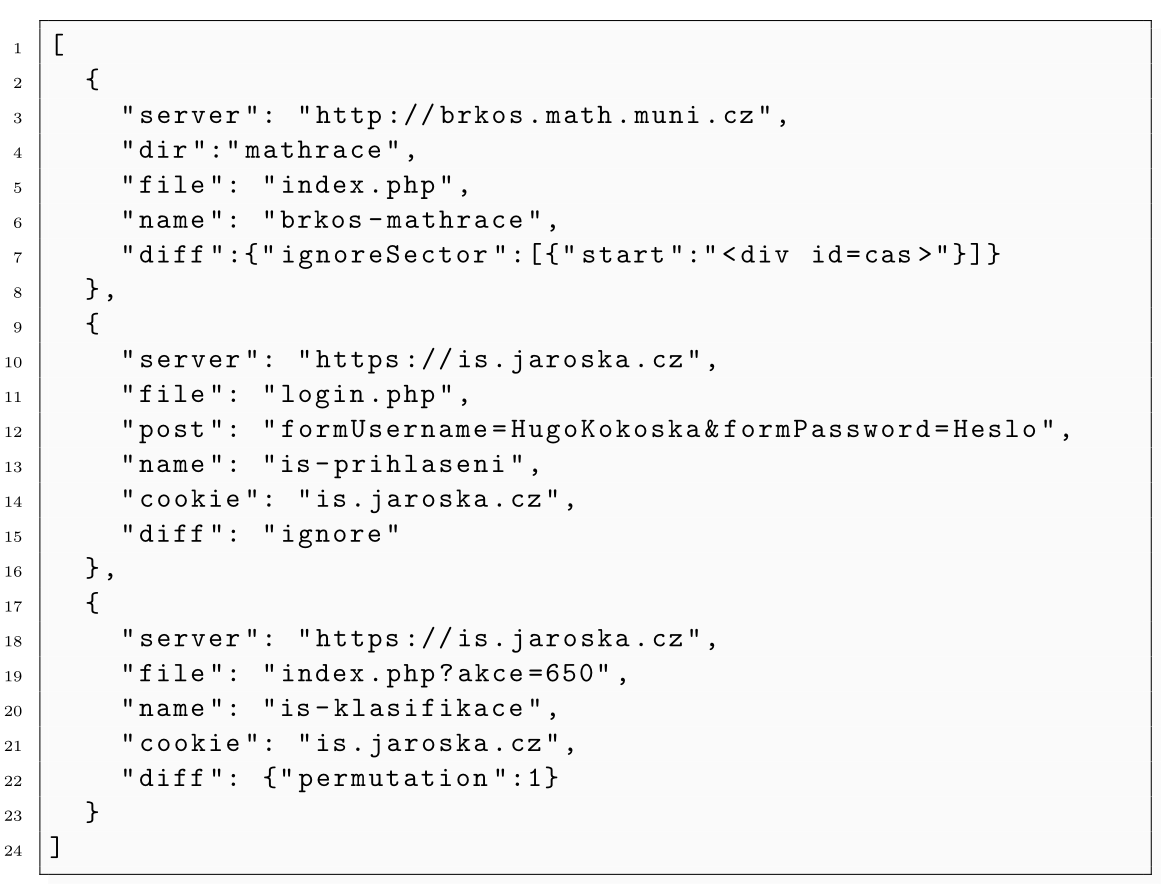
\includegraphics[width=10cm]{screenshots/config.png}
\end{center}
\end{frame}

\begin{frame}
  \frametitle{Main window}
\begin{center}
	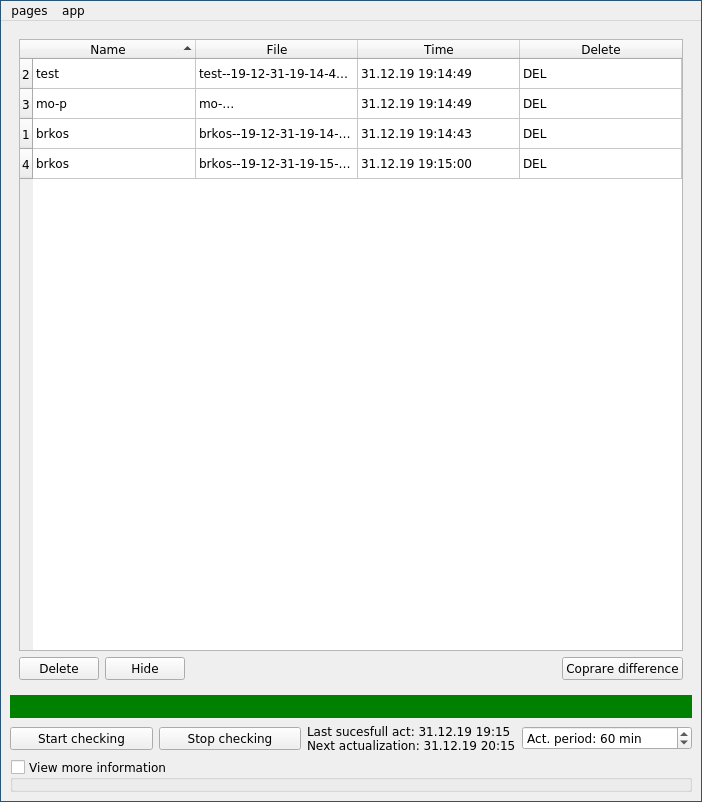
\includegraphics[width=6cm]{screenshots/basic_app2.png}
\end{center}
\end{frame}

\begin{frame}
  \frametitle{History window}
\begin{center}
	\includegraphics[width=9cm]{screenshots/history.png}
\end{center}
\end{frame}

\begin{frame}
  \frametitle{History window}
\begin{center}
	\includegraphics[width=11cm]{screenshots/compare.png}
\end{center}
\end{frame}

\section{Deploy}
\begin{frame}
  \frametitle{Qt}
\begin{center}
	
\includegraphics[width=4cm]{img/qt.png}
	\begin{block}{}
		Main library for application
	\end{block}
\end{center}
\end{frame}

\begin{frame}
  \frametitle{Qt creator}
\begin{center}
	\includegraphics[width=10cm]{screenshots/qtcreator.png}
\end{center}
\end{frame}
\begin{frame}
  \frametitle{Git}
\begin{center}
	
\includegraphics[width=10cm]{img/git.png}
	\begin{block}{}
		Version controller.
	\end{block}
\end{center}
\end{frame}

\begin{frame}
\section{Closing part}
\begin{center}
	\begin{block}{Free to use}
		Open source\\
		GNU LGPL licence
	\end{block}
	\begin{block}{Multiplatform}
		Linux (most of distribution)\\
		Windows\\
		(Mac OS)
	\end{block}
\end{center}
\end{frame}
\begin{frame}
\begin{center}
	\Huge Thank you for attention.
\end{center}
\end{frame}
\end{document}
